% Options for packages loaded elsewhere
\PassOptionsToPackage{unicode}{hyperref}
\PassOptionsToPackage{hyphens}{url}
%
\documentclass[
]{article}
\usepackage{amsmath,amssymb}
\usepackage{iftex}
\ifPDFTeX
  \usepackage[T1]{fontenc}
  \usepackage[utf8]{inputenc}
  \usepackage{textcomp} % provide euro and other symbols
\else % if luatex or xetex
  \usepackage{unicode-math} % this also loads fontspec
  \defaultfontfeatures{Scale=MatchLowercase}
  \defaultfontfeatures[\rmfamily]{Ligatures=TeX,Scale=1}
\fi
\usepackage{lmodern}
\ifPDFTeX\else
  % xetex/luatex font selection
\fi
% Use upquote if available, for straight quotes in verbatim environments
\IfFileExists{upquote.sty}{\usepackage{upquote}}{}
\IfFileExists{microtype.sty}{% use microtype if available
  \usepackage[]{microtype}
  \UseMicrotypeSet[protrusion]{basicmath} % disable protrusion for tt fonts
}{}
\makeatletter
\@ifundefined{KOMAClassName}{% if non-KOMA class
  \IfFileExists{parskip.sty}{%
    \usepackage{parskip}
  }{% else
    \setlength{\parindent}{0pt}
    \setlength{\parskip}{6pt plus 2pt minus 1pt}}
}{% if KOMA class
  \KOMAoptions{parskip=half}}
\makeatother
\usepackage{xcolor}
\usepackage[margin=1in]{geometry}
\usepackage{color}
\usepackage{fancyvrb}
\newcommand{\VerbBar}{|}
\newcommand{\VERB}{\Verb[commandchars=\\\{\}]}
\DefineVerbatimEnvironment{Highlighting}{Verbatim}{commandchars=\\\{\}}
% Add ',fontsize=\small' for more characters per line
\usepackage{framed}
\definecolor{shadecolor}{RGB}{248,248,248}
\newenvironment{Shaded}{\begin{snugshade}}{\end{snugshade}}
\newcommand{\AlertTok}[1]{\textcolor[rgb]{0.94,0.16,0.16}{#1}}
\newcommand{\AnnotationTok}[1]{\textcolor[rgb]{0.56,0.35,0.01}{\textbf{\textit{#1}}}}
\newcommand{\AttributeTok}[1]{\textcolor[rgb]{0.13,0.29,0.53}{#1}}
\newcommand{\BaseNTok}[1]{\textcolor[rgb]{0.00,0.00,0.81}{#1}}
\newcommand{\BuiltInTok}[1]{#1}
\newcommand{\CharTok}[1]{\textcolor[rgb]{0.31,0.60,0.02}{#1}}
\newcommand{\CommentTok}[1]{\textcolor[rgb]{0.56,0.35,0.01}{\textit{#1}}}
\newcommand{\CommentVarTok}[1]{\textcolor[rgb]{0.56,0.35,0.01}{\textbf{\textit{#1}}}}
\newcommand{\ConstantTok}[1]{\textcolor[rgb]{0.56,0.35,0.01}{#1}}
\newcommand{\ControlFlowTok}[1]{\textcolor[rgb]{0.13,0.29,0.53}{\textbf{#1}}}
\newcommand{\DataTypeTok}[1]{\textcolor[rgb]{0.13,0.29,0.53}{#1}}
\newcommand{\DecValTok}[1]{\textcolor[rgb]{0.00,0.00,0.81}{#1}}
\newcommand{\DocumentationTok}[1]{\textcolor[rgb]{0.56,0.35,0.01}{\textbf{\textit{#1}}}}
\newcommand{\ErrorTok}[1]{\textcolor[rgb]{0.64,0.00,0.00}{\textbf{#1}}}
\newcommand{\ExtensionTok}[1]{#1}
\newcommand{\FloatTok}[1]{\textcolor[rgb]{0.00,0.00,0.81}{#1}}
\newcommand{\FunctionTok}[1]{\textcolor[rgb]{0.13,0.29,0.53}{\textbf{#1}}}
\newcommand{\ImportTok}[1]{#1}
\newcommand{\InformationTok}[1]{\textcolor[rgb]{0.56,0.35,0.01}{\textbf{\textit{#1}}}}
\newcommand{\KeywordTok}[1]{\textcolor[rgb]{0.13,0.29,0.53}{\textbf{#1}}}
\newcommand{\NormalTok}[1]{#1}
\newcommand{\OperatorTok}[1]{\textcolor[rgb]{0.81,0.36,0.00}{\textbf{#1}}}
\newcommand{\OtherTok}[1]{\textcolor[rgb]{0.56,0.35,0.01}{#1}}
\newcommand{\PreprocessorTok}[1]{\textcolor[rgb]{0.56,0.35,0.01}{\textit{#1}}}
\newcommand{\RegionMarkerTok}[1]{#1}
\newcommand{\SpecialCharTok}[1]{\textcolor[rgb]{0.81,0.36,0.00}{\textbf{#1}}}
\newcommand{\SpecialStringTok}[1]{\textcolor[rgb]{0.31,0.60,0.02}{#1}}
\newcommand{\StringTok}[1]{\textcolor[rgb]{0.31,0.60,0.02}{#1}}
\newcommand{\VariableTok}[1]{\textcolor[rgb]{0.00,0.00,0.00}{#1}}
\newcommand{\VerbatimStringTok}[1]{\textcolor[rgb]{0.31,0.60,0.02}{#1}}
\newcommand{\WarningTok}[1]{\textcolor[rgb]{0.56,0.35,0.01}{\textbf{\textit{#1}}}}
\usepackage{graphicx}
\makeatletter
\def\maxwidth{\ifdim\Gin@nat@width>\linewidth\linewidth\else\Gin@nat@width\fi}
\def\maxheight{\ifdim\Gin@nat@height>\textheight\textheight\else\Gin@nat@height\fi}
\makeatother
% Scale images if necessary, so that they will not overflow the page
% margins by default, and it is still possible to overwrite the defaults
% using explicit options in \includegraphics[width, height, ...]{}
\setkeys{Gin}{width=\maxwidth,height=\maxheight,keepaspectratio}
% Set default figure placement to htbp
\makeatletter
\def\fps@figure{htbp}
\makeatother
\setlength{\emergencystretch}{3em} % prevent overfull lines
\providecommand{\tightlist}{%
  \setlength{\itemsep}{0pt}\setlength{\parskip}{0pt}}
\setcounter{secnumdepth}{-\maxdimen} % remove section numbering
\ifLuaTeX
  \usepackage{selnolig}  % disable illegal ligatures
\fi
\IfFileExists{bookmark.sty}{\usepackage{bookmark}}{\usepackage{hyperref}}
\IfFileExists{xurl.sty}{\usepackage{xurl}}{} % add URL line breaks if available
\urlstyle{same}
\hypersetup{
  pdftitle={Proyecto\_completo},
  pdfauthor={Larissa Cordero},
  hidelinks,
  pdfcreator={LaTeX via pandoc}}

\title{Proyecto\_completo}
\author{Larissa Cordero}
\date{2023-10-24}

\begin{document}
\maketitle

\hypertarget{resultados-muestras-vid-peruxfa}{%
\section{Resultados muestras vid
Perú}\label{resultados-muestras-vid-peruxfa}}

\hypertarget{anuxe1lisis-actividad-enzimuxe1tica-conteo-total-de-hongos-y-bacterias.}{%
\subsection{\texorpdfstring{\emph{Análisis:} Actividad Enzimática,
Conteo total de hongos y
Bacterias.}{Análisis: Actividad Enzimática, Conteo total de hongos y Bacterias.}}\label{anuxe1lisis-actividad-enzimuxe1tica-conteo-total-de-hongos-y-bacterias.}}

\hypertarget{librerias}{%
\paragraph{Librerias}\label{librerias}}

\begin{Shaded}
\begin{Highlighting}[]
\FunctionTok{library}\NormalTok{(dplyr)}
\FunctionTok{library}\NormalTok{(tidyverse)}
\FunctionTok{library}\NormalTok{(car)}
\FunctionTok{library}\NormalTok{(agricolae)}
\FunctionTok{library}\NormalTok{(latexpdf)}
\FunctionTok{library}\NormalTok{(tinytex)}
\FunctionTok{library}\NormalTok{(devtools)}
\NormalTok{devtools}\SpecialCharTok{::}\FunctionTok{install\_github}\NormalTok{(}\StringTok{\textquotesingle{}yihui/tinytex\textquotesingle{}}\NormalTok{)}
\end{Highlighting}
\end{Shaded}

\begin{verbatim}
## 
## -- R CMD build -----------------------------------------------------------------
##          checking for file 'C:\Users\lcordero\AppData\Local\Temp\Rtmpmon6V6\remotes2b04289370c\rstudio-tinytex-3495cb8/DESCRIPTION' ...     checking for file 'C:\Users\lcordero\AppData\Local\Temp\Rtmpmon6V6\remotes2b04289370c\rstudio-tinytex-3495cb8/DESCRIPTION' ...   v  checking for file 'C:\Users\lcordero\AppData\Local\Temp\Rtmpmon6V6\remotes2b04289370c\rstudio-tinytex-3495cb8/DESCRIPTION' (669ms)
##       -  preparing 'tinytex': (678ms)
##    checking DESCRIPTION meta-information ...     checking DESCRIPTION meta-information ...   v  checking DESCRIPTION meta-information
##       -  checking for LF line-endings in source and make files and shell scripts
##   -  checking for empty or unneeded directories
##   -  building 'tinytex_0.48.2.tar.gz'
##      
## 
\end{verbatim}

\begin{verbatim}
## Warning: package 'tinytex' is in use and will not be installed
\end{verbatim}

\hypertarget{datos}{%
\paragraph{Datos}\label{datos}}

\begin{Shaded}
\begin{Highlighting}[]
\NormalTok{Resultados }\OtherTok{\textless{}{-}} \FunctionTok{read.csv}\NormalTok{(}\StringTok{"\textasciitilde{}/capR/curso/curso\_Innovak/Proyecto/Datos/Muestras\_peru.csv"}\NormalTok{)}

\NormalTok{Estanque\_de\_plantas }\OtherTok{\textless{}{-}} \FunctionTok{read.csv}\NormalTok{(}\StringTok{"\textasciitilde{}/capR/curso/curso\_Innovak/Material\_clase/Estanque\_plantas.csv"}\NormalTok{)}
\end{Highlighting}
\end{Shaded}

\emph{Verificación de datos}

\begin{Shaded}
\begin{Highlighting}[]
\CommentTok{\# Actividad\_enzimatica}

\FunctionTok{hist}\NormalTok{(Resultados}\SpecialCharTok{$}\NormalTok{Actividad.\_enzimatica)}
\end{Highlighting}
\end{Shaded}

\includegraphics{Proyecto_completo_files/figure-latex/unnamed-chunk-3-1.pdf}

\begin{Shaded}
\begin{Highlighting}[]
\FunctionTok{qqnorm}\NormalTok{(Resultados}\SpecialCharTok{$}\NormalTok{Actividad.\_enzimatica)}
\end{Highlighting}
\end{Shaded}

\includegraphics{Proyecto_completo_files/figure-latex/unnamed-chunk-3-2.pdf}

\begin{Shaded}
\begin{Highlighting}[]
\FunctionTok{shapiro.test}\NormalTok{(Resultados}\SpecialCharTok{$}\NormalTok{Actividad.\_enzimatica)}
\end{Highlighting}
\end{Shaded}

\begin{verbatim}
## 
##  Shapiro-Wilk normality test
## 
## data:  Resultados$Actividad._enzimatica
## W = 0.94319, p-value = 0.09226
\end{verbatim}

\begin{Shaded}
\begin{Highlighting}[]
\CommentTok{\# Hongos\_totales}

\FunctionTok{hist}\NormalTok{(Resultados}\SpecialCharTok{$}\NormalTok{Hongos\_totales)}
\end{Highlighting}
\end{Shaded}

\includegraphics{Proyecto_completo_files/figure-latex/unnamed-chunk-3-3.pdf}

\begin{Shaded}
\begin{Highlighting}[]
\FunctionTok{qqnorm}\NormalTok{(Resultados}\SpecialCharTok{$}\NormalTok{Hongos\_totales)}
\end{Highlighting}
\end{Shaded}

\includegraphics{Proyecto_completo_files/figure-latex/unnamed-chunk-3-4.pdf}

\begin{Shaded}
\begin{Highlighting}[]
\FunctionTok{shapiro.test}\NormalTok{(Resultados}\SpecialCharTok{$}\NormalTok{Hongos\_totales) }
\end{Highlighting}
\end{Shaded}

\begin{verbatim}
## 
##  Shapiro-Wilk normality test
## 
## data:  Resultados$Hongos_totales
## W = 0.90174, p-value = 0.006859
\end{verbatim}

\begin{Shaded}
\begin{Highlighting}[]
\CommentTok{\# Bacterias\_totales }

\FunctionTok{hist}\NormalTok{(Resultados}\SpecialCharTok{$}\NormalTok{Bacterias\_totales)}
\end{Highlighting}
\end{Shaded}

\includegraphics{Proyecto_completo_files/figure-latex/unnamed-chunk-3-5.pdf}

\begin{Shaded}
\begin{Highlighting}[]
\FunctionTok{qqnorm}\NormalTok{(Resultados}\SpecialCharTok{$}\NormalTok{Bacterias\_totales)}
\end{Highlighting}
\end{Shaded}

\includegraphics{Proyecto_completo_files/figure-latex/unnamed-chunk-3-6.pdf}

\begin{Shaded}
\begin{Highlighting}[]
\FunctionTok{shapiro.test}\NormalTok{(Resultados}\SpecialCharTok{$}\NormalTok{Bacterias\_totales) }
\end{Highlighting}
\end{Shaded}

\begin{verbatim}
## 
##  Shapiro-Wilk normality test
## 
## data:  Resultados$Bacterias_totales
## W = 0.91461, p-value = 0.01489
\end{verbatim}

\begin{Shaded}
\begin{Highlighting}[]
\CommentTok{\# Normalizar datos }

\FunctionTok{shapiro.test}\NormalTok{(}\FunctionTok{log}\NormalTok{(Resultados}\SpecialCharTok{$}\NormalTok{Bacterias\_totales)) }
\end{Highlighting}
\end{Shaded}

\begin{verbatim}
## 
##  Shapiro-Wilk normality test
## 
## data:  log(Resultados$Bacterias_totales)
## W = 0.91846, p-value = 0.01888
\end{verbatim}

\begin{Shaded}
\begin{Highlighting}[]
\FunctionTok{hist}\NormalTok{(}\FunctionTok{log}\NormalTok{(Resultados}\SpecialCharTok{$}\NormalTok{Bacterias\_totales))}
\end{Highlighting}
\end{Shaded}

\includegraphics{Proyecto_completo_files/figure-latex/unnamed-chunk-3-7.pdf}

\begin{Shaded}
\begin{Highlighting}[]
\FunctionTok{qqnorm}\NormalTok{(}\FunctionTok{log}\NormalTok{(Resultados}\SpecialCharTok{$}\NormalTok{Bacterias\_totales))}
\end{Highlighting}
\end{Shaded}

\includegraphics{Proyecto_completo_files/figure-latex/unnamed-chunk-3-8.pdf}

\begin{Shaded}
\begin{Highlighting}[]
\CommentTok{\# Verificar el balance de los datos}

\NormalTok{Resultados }\SpecialCharTok{\%\textgreater{}\%}
  \FunctionTok{group\_by}\NormalTok{(Variedad) }\SpecialCharTok{\%\textgreater{}\%}
  \FunctionTok{summarise}\NormalTok{ (}\FunctionTok{n}\NormalTok{())}
\end{Highlighting}
\end{Shaded}

\begin{verbatim}
## # A tibble: 2 x 2
##   Variedad     `n()`
##   <chr>        <int>
## 1 Cotton candy    16
## 2 Sweet globe     16
\end{verbatim}

\begin{Shaded}
\begin{Highlighting}[]
\CommentTok{\# Homogenidad de varianza}


\FunctionTok{leveneTest}\NormalTok{(}\FunctionTok{log}\NormalTok{(Bacterias\_totales) }\SpecialCharTok{\textasciitilde{}}\NormalTok{ Variedad}\SpecialCharTok{*}\NormalTok{Tipo\_muestra, }\AttributeTok{data =}\NormalTok{ Resultados) }\CommentTok{\# no hay homogeneidad}
\end{Highlighting}
\end{Shaded}

\begin{verbatim}
## Levene's Test for Homogeneity of Variance (center = median)
##       Df F value  Pr(>F)  
## group  3  4.5045 0.01062 *
##       28                  
## ---
## Signif. codes:  0 '***' 0.001 '**' 0.01 '*' 0.05 '.' 0.1 ' ' 1
\end{verbatim}

\begin{Shaded}
\begin{Highlighting}[]
\FunctionTok{leveneTest}\NormalTok{(Actividad.\_enzimatica }\SpecialCharTok{\textasciitilde{}}\NormalTok{ Variedad}\SpecialCharTok{*}\NormalTok{Tipo\_muestra, }\AttributeTok{data =}\NormalTok{ Resultados) }\CommentTok{\# si hay homogeneidad}
\end{Highlighting}
\end{Shaded}

\begin{verbatim}
## Levene's Test for Homogeneity of Variance (center = median)
##       Df F value Pr(>F)
## group  3  0.7426 0.5357
##       28
\end{verbatim}

\hypertarget{los-resultados-de-verificaciuxf3n-son-los-siguientes}{%
\subsubsection{Los resultados de verificación son los
siguientes:}\label{los-resultados-de-verificaciuxf3n-son-los-siguientes}}

\hypertarget{actividad_enzimatica}{%
\paragraph{\texorpdfstring{\textbf{Actividad\_enzimatica}:}{Actividad\_enzimatica:}}\label{actividad_enzimatica}}

\emph{Shapiro}= 0.09226 Conforme a los resultados de shapiro, es
\textgreater0.05, por lo cual ya estan normalizados los datos y también
con las graficas se puede observar que si.

\hypertarget{bacterias_totales}{%
\paragraph{\texorpdfstring{\textbf{Bacterias\_totales}:}{Bacterias\_totales:}}\label{bacterias_totales}}

\emph{Shapiro}=0.01489 Conforme a los resultados de shapiro, es
\textless0.05, por lo cual es necesario transformar los datos, y en la
grafica se observa que tiene un sesgo a la derecha por lo que utilcé log
para normalizarlos.

\hypertarget{balance-de-datos}{%
\paragraph{\texorpdfstring{\textbf{Balance de
datos}:}{Balance de datos:}}\label{balance-de-datos}}

Es importante verificar que se cuente con el mismo numero de datos, en
este analisis se cuenta con 16 datos para la variedad \emph{cotton
candy} y 16 para \emph{sweet globe}

\hypertarget{homogeneidad-de-varianza}{%
\paragraph{\texorpdfstring{\textbf{Homogeneidad de
varianza}:}{Homogeneidad de varianza:}}\label{homogeneidad-de-varianza}}

Se realizó la prueba de Levene arrojando los siguientes resultados

1.\emph{Bacterias\_totales}: p= 0.01062 2.\emph{Actividad\_ezimatica}:p
= 0.5357

\hypertarget{con-los-resultados-anteriores-se-concluye-que-si-hay-homogeneidad-con-los-datos-de-actividad-enzimatica-y-que-con-la-interacciuxf3n-de-los-datos-con-bacterias_totales-no-hay-homogeneidad.}{%
\subparagraph{Con los resultados anteriores se concluye que si hay
homogeneidad con los datos de actividad enzimatica y que con la
interacción de los datos con Bacterias\_totales no hay
homogeneidad.}\label{con-los-resultados-anteriores-se-concluye-que-si-hay-homogeneidad-con-los-datos-de-actividad-enzimatica-y-que-con-la-interacciuxf3n-de-los-datos-con-bacterias_totales-no-hay-homogeneidad.}}

\hypertarget{anova}{%
\subsubsection{\texorpdfstring{\textbf{ANOVA}}{ANOVA}}\label{anova}}

\begin{Shaded}
\begin{Highlighting}[]
\CommentTok{\# Anova dos vías}

\NormalTok{Anova\_enz }\OtherTok{\textless{}{-}} \FunctionTok{aov}\NormalTok{(Actividad.\_enzimatica }\SpecialCharTok{\textasciitilde{}}\NormalTok{ Variedad}\SpecialCharTok{*}\NormalTok{Tipo\_muestra, }\AttributeTok{data =}\NormalTok{ Resultados)}

\FunctionTok{Anova}\NormalTok{(Anova\_enz)}
\end{Highlighting}
\end{Shaded}

\begin{verbatim}
## Anova Table (Type II tests)
## 
## Response: Actividad._enzimatica
##                        Sum Sq Df F value   Pr(>F)    
## Variedad                4.247  1  2.2421   0.1455    
## Tipo_muestra          126.769  1 66.9227 6.63e-09 ***
## Variedad:Tipo_muestra   2.847  1  1.5029   0.2304    
## Residuals              53.039 28                     
## ---
## Signif. codes:  0 '***' 0.001 '**' 0.01 '*' 0.05 '.' 0.1 ' ' 1
\end{verbatim}

\begin{Shaded}
\begin{Highlighting}[]
\CommentTok{\# Prueba Tukey}

\NormalTok{Anova\_tukey }\OtherTok{\textless{}{-}} \FunctionTok{TukeyHSD}\NormalTok{(Anova\_enz)}
\FunctionTok{plot}\NormalTok{(Anova\_tukey)}
\end{Highlighting}
\end{Shaded}

\includegraphics{Proyecto_completo_files/figure-latex/unnamed-chunk-4-1.pdf}
\includegraphics{Proyecto_completo_files/figure-latex/unnamed-chunk-4-2.pdf}
\includegraphics{Proyecto_completo_files/figure-latex/unnamed-chunk-4-3.pdf}

\begin{Shaded}
\begin{Highlighting}[]
\FunctionTok{summary}\NormalTok{(Anova\_enz)}
\end{Highlighting}
\end{Shaded}

\begin{verbatim}
##                       Df Sum Sq Mean Sq F value   Pr(>F)    
## Variedad               1   4.25    4.25   2.242    0.145    
## Tipo_muestra           1 126.77  126.77  66.923 6.63e-09 ***
## Variedad:Tipo_muestra  1   2.85    2.85   1.503    0.230    
## Residuals             28  53.04    1.89                     
## ---
## Signif. codes:  0 '***' 0.001 '**' 0.01 '*' 0.05 '.' 0.1 ' ' 1
\end{verbatim}

\begin{Shaded}
\begin{Highlighting}[]
\NormalTok{grupos }\OtherTok{\textless{}{-}} \FunctionTok{HSD.test}\NormalTok{(Anova\_enz, }\AttributeTok{trt =} \FunctionTok{c}\NormalTok{(}\StringTok{"Variedad"}\NormalTok{,}\StringTok{"Tipo\_muestra"}\NormalTok{),}
                  \AttributeTok{alpha =} \FloatTok{0.05}\NormalTok{)}
\end{Highlighting}
\end{Shaded}

\hypertarget{interpretaciuxf3n-resultados}{%
\subsubsection{\texorpdfstring{\textbf{Interpretación
resultados}}{Interpretación resultados}}\label{interpretaciuxf3n-resultados}}

\hypertarget{conforme-a-los-resultados-obtenidos-en-la-prueba-de-tukey-se-interpreta-de-la-siguiente-manera}{%
\paragraph{Conforme a los resultados obtenidos en la prueba de Tukey se
interpreta de la siguiente
manera:}\label{conforme-a-los-resultados-obtenidos-en-la-prueba-de-tukey-se-interpreta-de-la-siguiente-manera}}

\begin{enumerate}
\def\labelenumi{\arabic{enumi}.}
\item
  En las muestras de los tipos de variedades da un valor p = 0.145 por
  lo que \textbf{no} hay diferencias significativas entre la variedad
  \emph{Sweet globe} y \emph{Cotton candy}
\item
  En las muestras de los tipos da un valor de p = 6.63e-09, por lo que
  aquí \textbf{si} hay diferencias significativas en las muestras
  \emph{testigo} y \emph{tratadas}
\item
  En la interacción de las muestras de variedad con el tipo ya sea
  testigo o tratado \textbf{no} hay diferencia significativa ya que el
  valor de p = 0.230
\end{enumerate}

\hypertarget{separar-por-grupos}{%
\paragraph{Separar por grupos}\label{separar-por-grupos}}

\hypertarget{tambiuxe9n-se-corriuxf3-el-anuxe1lisis-donde-separa-por-grupos-se-puede-observar-en-la-siguiente-tabla}{%
\paragraph{También se corrió el análisis donde separa por grupos, se
puede observar en la siguiente
tabla:}\label{tambiuxe9n-se-corriuxf3-el-anuxe1lisis-donde-separa-por-grupos-se-puede-observar-en-la-siguiente-tabla}}

\begin{figure}
\centering
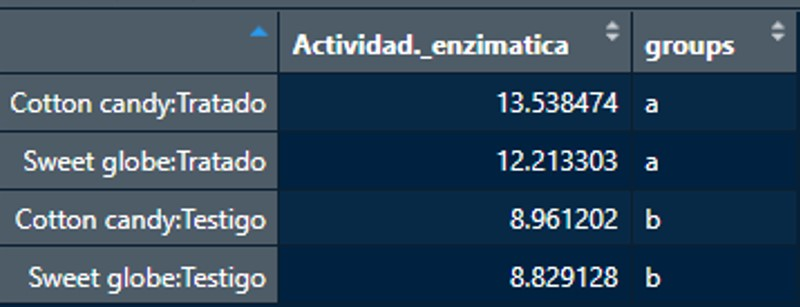
\includegraphics{Imagen1.jpg}
\caption{Tabla1}
\end{figure}

\hypertarget{el-grupo-a-correponde-a-los-tratados-en-los-cuales-no-hay-diferencia-significativa-y-el-grupo-b-corresponde-a-los-testigos-por-lo-que-se-concluye-lo-mismo-que-se-menciona-anteriormente-que-si-existe-una-diferencia-entre-el-grupo-a-y-b-testigos-y-tratados-pero-en-la-variedad-no-hay-diferencia.}{%
\paragraph{\texorpdfstring{El grupo \textbf{A} correponde a los tratados
en los cuales no hay diferencia significativa, y el grupo \textbf{B}
corresponde a los testigos, por lo que se concluye lo mismo que se
menciona anteriormente que \textbf{si} existe una diferencia entre el
grupo A y B \textbf{Testigos y Tratados}, pero en la variedad no hay
diferencia.}{El grupo A correponde a los tratados en los cuales no hay diferencia significativa, y el grupo B corresponde a los testigos, por lo que se concluye lo mismo que se menciona anteriormente que si existe una diferencia entre el grupo A y B Testigos y Tratados, pero en la variedad no hay diferencia.}}\label{el-grupo-a-correponde-a-los-tratados-en-los-cuales-no-hay-diferencia-significativa-y-el-grupo-b-corresponde-a-los-testigos-por-lo-que-se-concluye-lo-mismo-que-se-menciona-anteriormente-que-si-existe-una-diferencia-entre-el-grupo-a-y-b-testigos-y-tratados-pero-en-la-variedad-no-hay-diferencia.}}

\hypertarget{las-muestras-testigo-pertenecen-a-muestras-de-suelo-sin-aplicaciuxf3n-de-producto-bioluxf3gico-y-las-muestras-tratadas-fueron-aplicadas-con-el-producto-y-si-hay-un-aumento-de-la-actividad-enzimatica-aplicando-el-tratamiento-por-lo-cual-estuxe1-relacionado-al-incremento-de-microorgnismos-en-suelo.}{%
\paragraph{Las muestras testigo pertenecen a muestras de suelo sin
aplicación de producto biológico y las muestras tratadas fueron
aplicadas con el producto y si hay un aumento de la actividad enzimatica
aplicando el tratamiento por lo cual está relacionado al incremento de
microorgnismos en
suelo.}\label{las-muestras-testigo-pertenecen-a-muestras-de-suelo-sin-aplicaciuxf3n-de-producto-bioluxf3gico-y-las-muestras-tratadas-fueron-aplicadas-con-el-producto-y-si-hay-un-aumento-de-la-actividad-enzimatica-aplicando-el-tratamiento-por-lo-cual-estuxe1-relacionado-al-incremento-de-microorgnismos-en-suelo.}}

\hypertarget{para-conocer-muxe1s-sobre-que-es-un-anuxe1lisis-de-varianza-tipo-anova-a-informacion-la-pueden-encontrar-en-el-siguiente-link}{%
\paragraph{Para conocer más sobre que es un análisis de varianza tipo
ANOVA, a informacion la pueden encontrar en el siguiente
link:}\label{para-conocer-muxe1s-sobre-que-es-un-anuxe1lisis-de-varianza-tipo-anova-a-informacion-la-pueden-encontrar-en-el-siguiente-link}}

\href{https://rpubs.com/Joaquin_AR/219148}{Mas información}

\hypertarget{se-utilizuxf3-el-codigo-de-shapiro-para-transformar-el-valor-de-los-datos}{%
\subsubsection{Se utilizó el codigo de shapiro para transformar el valor
de los
datos}\label{se-utilizuxf3-el-codigo-de-shapiro-para-transformar-el-valor-de-los-datos}}

\begin{Shaded}
\begin{Highlighting}[]
\CommentTok{\# Cambiar el valor de los resultados de Actividad enzimatica de ug a mg}

\ControlFlowTok{for}\NormalTok{ (i }\ControlFlowTok{in} \DecValTok{1}\SpecialCharTok{:} \FunctionTok{nrow}\NormalTok{(Resultados)) \{}
\NormalTok{  enz\_mg }\OtherTok{\textless{}{-}}\NormalTok{ Resultados}\SpecialCharTok{$}\NormalTok{Actividad.\_enzimatica[i]}\SpecialCharTok{/}\DecValTok{1000}
  \FunctionTok{print}\NormalTok{(enz\_mg)}
\NormalTok{\}}
\end{Highlighting}
\end{Shaded}

\begin{verbatim}
## [1] 0.007550459
## [1] 0.007321101
## [1] 0.008743119
## [1] 0.008513761
## [1] 0.009844037
## [1] 0.009889908
## [1] 0.009385321
## [1] 0.009385321
## [1] 0.008146789
## [1] 0.008330275
## [1] 0.008055046
## [1] 0.008605505
## [1] 0.008055046
## [1] 0.01034862
## [1] 0.009295122
## [1] 0.01085321
## [1] 0.01456881
## [1] 0.01080734
## [1] 0.012
## [1] 0.01507339
## [1] 0.0126422
## [1] 0.01088991
## [1] 0.01033945
## [1] 0.01138532
## [1] 0.01305505
## [1] 0.01342202
## [1] 0.01122008
## [1] 0.0124556
## [1] 0.01280309
## [1] 0.01562162
## [1] 0.01546718
## [1] 0.01426316
\end{verbatim}

\hypertarget{ejercicio}{%
\subsection{Ejercicio}\label{ejercicio}}

\hypertarget{determinar-si-existe-una-correlaciuxf3n-entre-la-biomasa-de-dos-especies-acuuxe1ticas-de-plantas-en-estanques-de-alaska-carex-y-artophila-usando-datos-modernos.}{%
\subsubsection{Determinar si existe una correlación entre la biomasa de
dos especies acuáticas de plantas en estanques de Alaska: Carex y
Artophila, usando datos
modernos.}\label{determinar-si-existe-una-correlaciuxf3n-entre-la-biomasa-de-dos-especies-acuuxe1ticas-de-plantas-en-estanques-de-alaska-carex-y-artophila-usando-datos-modernos.}}

\begin{Shaded}
\begin{Highlighting}[]
\CommentTok{\# Seleccionar columnas que vamos a utilizar para el analisis }

\NormalTok{Tmodificada }\OtherTok{\textless{}{-}}\NormalTok{ Estanque\_de\_plantas[,}\FunctionTok{c}\NormalTok{(}\StringTok{"Era"}\NormalTok{, }\StringTok{"Artophila"}\NormalTok{, }\StringTok{"Carex"}\NormalTok{)]}

\NormalTok{Modificada }\OtherTok{\textless{}{-}}\NormalTok{ Tmodificada }\SpecialCharTok{\%\textgreater{}\%}
  \FunctionTok{filter}\NormalTok{(}\SpecialCharTok{!}\FunctionTok{is.na}\NormalTok{(Artophila),}\SpecialCharTok{!}\FunctionTok{is.na}\NormalTok{(Carex)) }\SpecialCharTok{\%\textgreater{}\%}
  \FunctionTok{select}\NormalTok{(Era, Artophila, Carex)}
   

\CommentTok{\# Verificar si cumple con las funciones }

\FunctionTok{plot}\NormalTok{(Modificada}\SpecialCharTok{$}\NormalTok{Artophila,Modificada}\SpecialCharTok{$}\NormalTok{Carex)}
\end{Highlighting}
\end{Shaded}

\includegraphics{Proyecto_completo_files/figure-latex/unnamed-chunk-6-1.pdf}

\begin{Shaded}
\begin{Highlighting}[]
\DocumentationTok{\#\# Correlacion }

\FunctionTok{cor.test}\NormalTok{(Modificada}\SpecialCharTok{$}\NormalTok{Artophila,Modificada}\SpecialCharTok{$}\NormalTok{Carex)}
\end{Highlighting}
\end{Shaded}

\begin{verbatim}
## 
##  Pearson's product-moment correlation
## 
## data:  Modificada$Artophila and Modificada$Carex
## t = 3.6467, df = 17, p-value = 0.001996
## alternative hypothesis: true correlation is not equal to 0
## 95 percent confidence interval:
##  0.2979541 0.8584059
## sample estimates:
##       cor 
## 0.6625044
\end{verbatim}

\hypertarget{resultados}{%
\paragraph{Resultados}\label{resultados}}

\hypertarget{el-coeficiente-de-correlaciuxf3n-da-un-valor-de-0.6625044-y-el-p-value-0.001996-por-lo-que-se-considera-que-la-correlaciuxf3n-es-significativa-ya-que-para-considerar-eso-es-necesario-que-el-valor-de-p-value-sea-0.05}{%
\paragraph{El coeficiente de correlación da un valor de 0.6625044 y el
p-value =0.001996, por lo que se considera que la correlación es
significativa ya que para considerar eso es necesario que el valor de
p-value sea
\textless0.05}\label{el-coeficiente-de-correlaciuxf3n-da-un-valor-de-0.6625044-y-el-p-value-0.001996-por-lo-que-se-considera-que-la-correlaciuxf3n-es-significativa-ya-que-para-considerar-eso-es-necesario-que-el-valor-de-p-value-sea-0.05}}

\end{document}
